
% -*- TeX-master: "../dipole_ilya_paper.tex" -*-
\section{Operations with qubits}
\label{sec:characterisation}

% \red{Need scattering data}

\noindent We record the energy spectrum of  the twin qubit while sweeping the biasing magnetic
flux.  Because of a  small asymmetry, $\eta$, the fluxes linked through the  left and right loops
are $ \Phi = \frac{\varphi}{2\pi}\Phi_0$ and $ \eta\Phi $.

The \iket{1}~\ilra~\iket{2}  transition, $\omega_{21}$,  is mapped with  a network  analyzer, which
measures the transmission  of signal $\omega_{\text{NA}}$ through the system.   Away from resonance
the signal passes through the circuit without any interaction with the qubit. After correcting
for   line   losses,  transmission   is   close   to  $   100\%   $.    Only  near   resonance
($\omega_{\text{NA}}=\omega_{21}$), does the qubit exchange photons with the driving field as it evolves
between the ground and excited states \cite{rabi}.  The  qubit emits a wave that is exactly in
anti-phase with the driving field \cite{abdumalikov2010}, and the destructive superposition in
the output line results in a transmission dip, see Fig.~\ref{fig:transmission}.  The bottom of
this dip is marked with blue circles. The trace of circles at different magnetic flux maps out
the qubit's $\omega_{21}$ transition spectrum, see inset of Fig.~\ref{fig:transmission}.

\begin{figure}[h]
  \centering 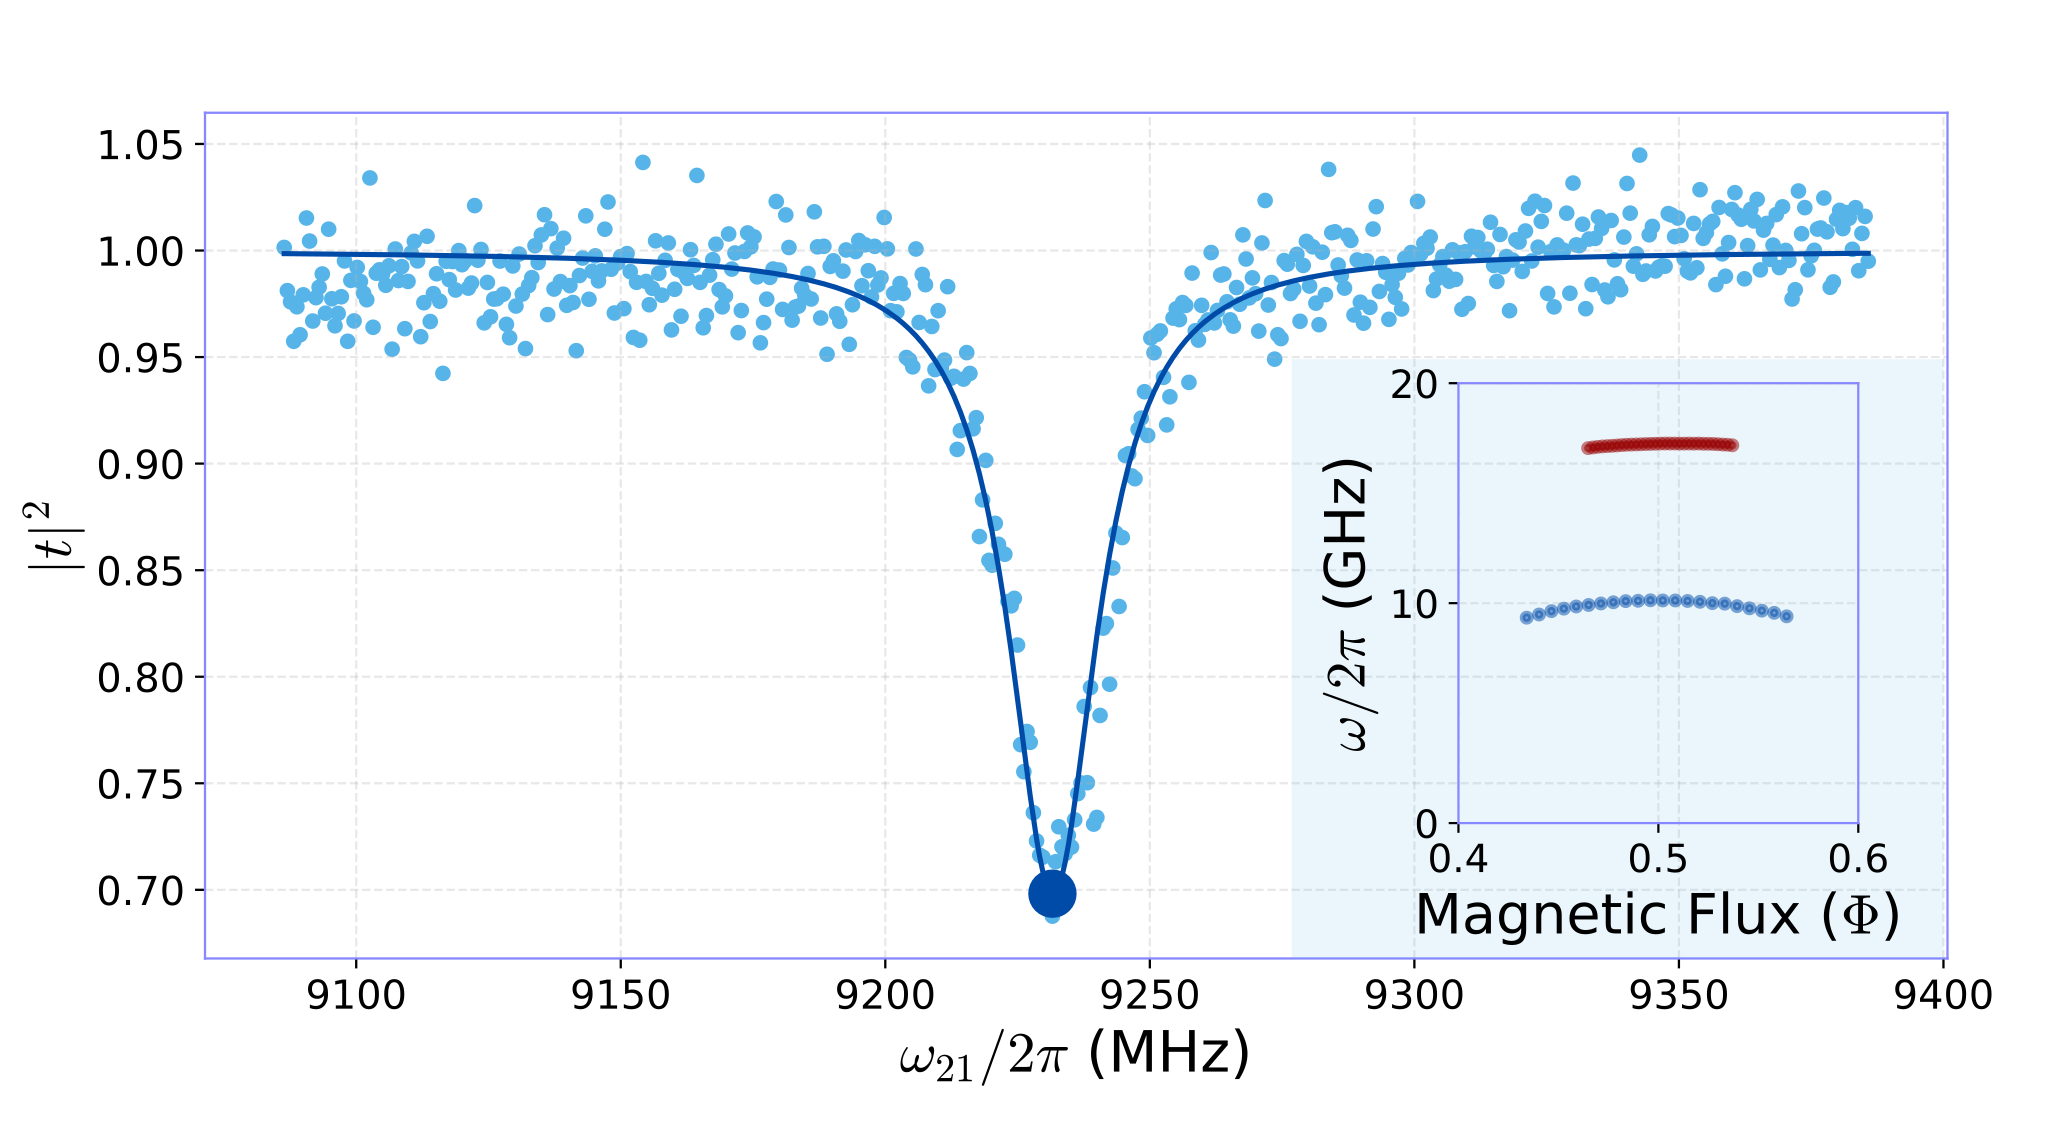
\includegraphics[height = 4.8cm]{fig2.png}
  \caption{\small \textbf{Mapping  the qubit transition  spectrum:}  For the  lower transition
    $\omega_{21}$ (blue,  inset) a  network analyzer measures  the power  transmission coefficient,
    \iabsSquared{t}, at flux  bias $ \Phi $  and microwave frequency $  \omega_{21}/2\pi$.  A Lorentzian
    fit \cite{Astafiev2010}  to the transmission  profile establishes the  resonant frequency,
    which  is  marked  with  blue  points on  the  flux-frequency  spectrum.   For  transition
    $\omega_{32}$  (red, inset)  a two-tone  measurement is  run by  monitoring changes  to a  weak
    $\omega_{21}$ probe while sweeping a second frequency  in search of the higher transition.
    % Any changes to the probe's transmission are indicative of hitting the higher transition, which
    % is marked with a red point on the spectrum.
    % Readings are taken about the degeneracy point
    % $  \Phi \sim  \Phi_{0}/2 $,  where the  low  curvature of  transition energies,  allows for  stable
    % measurements with respect to fluctuations in the field.
  }
  \label{fig:transmission}
\end{figure}

The \iket{2}\ilra\iket{3}  transition, $\omega_{32}$, is  mapped using two-tone  spectroscopy.  The
network  analyzer is  tuned to  the transition  frequency  $ \omega_{21}  $, taken  from the  first
measurement  and called  the  probe signal,  while  an additional  generator  sweeps a  second
frequency,  $  \omega_{\text{GEN}} $.   Whenever  the  generator strikes  the  \iket{2}\ira\iket{3}
transition ($\omega_{\text{GEN}} = \omega_{32} $), the qubit undergoes a ladder of excitations, \iket{1}
\iratext{$\omega_{21}$}\iket{2}  \iratext{$\omega_{32}$}  \iket{3},  depopulating  states  \iket{1}  and
\iket{2}.  Because of  this depopulation, the probe signal becomes  less involved with driving
and it's  transmission moves out of  the dip in Fig.~\ref{fig:transmission}.   This identifies
$\omega_{32}$ which is mapped with red circles in the transition energy-magnetic field spectrum.

% prove that state 1 becomes depopulated by solving the master equation for two drives

We  match the  experimental  data points  to  simulations made  on  the standard  Hamiltonian,
$  \mathcal{H}   =  T   +  U   $  \cite{orlando1999}.    Islands,  isolated   by  the   JJ  in
Fig.~\ref{fig:setup},     are     labeled     with     Cooper     pair     (CP)     occupation
$         \vec{n}        =         \iket{n_1,        n_2,         n_3}        $,         phase
$       \vec{\varphi}       =       \iket{\varphi_1,       \varphi_2,       \varphi_3}       $       and       voltage
$ \vec{V} = \iket{V_{1}, V_{2}, V_{3}} $ states.   The charges and voltages on the islands are
linked by the capacitance matrix
\begin{equation}
  \label{eq:link}
  2e\vec{n} = \hat{C}\vec{V}
\end{equation}

\noindent where the capacitance matrix in the topology of Fig.~\ref{fig:setup} is
\begin{equation}
  \label{eq:capac}
  \hat{C} = \iabs{C} \begin{pmatrix}
    2  &  -1  &  0\\
    -1  &  2  +  \alpha  &  -1\\
    0  &  -1  & 2
  \end{pmatrix},
\end{equation}

\noindent where  \iabs{C} is the capacitance  of the outer  JJs.  The interaction of  the CPs,
carrying a charge $  \vec{Q}=2e\vec{n} $, and voltages on their  respective islands gives rise
to the `kinetic' term of the Hamiltonian:
\begin{equation}\label{eq:kinetic}
  \begin{aligned}
    T = \frac{1}{2}\sum_{i=1}^{3}Q_iV_i & =
    \frac{(2e)^2}{2}\vec{n}\hat{C}^{-1}\vec{n}^{T}\\
    & = E_C \iabs{C} \iaverage{\hat{C}^{-1}}_{\iket{n_{1}, n_2, n_3}},
  \end{aligned}
\end{equation}

\noindent where we define $ E_{C}={(2e)^{2}}/{2 \iabs{C} } $.

Each  JJ  with   a  phase  difference  of  $\Delta\varphi_{i}$,  contributes   a  `potential'  energy  of
$ E_{Ji}\left(1 - \cos(\Delta\varphi_i)\right) $.  The flux quantization condition for the left and right
loops,  $  \sum_{i}^{\text{loop}} \varphi_i  =  2\pi  n,  n \in  \mathbb{Z}$,  enters  as a  dependence  on
$ \varphi_\text{ext} $ and $ \eta\varphi_\text{ext} $ on two of the junctions:
\begin{equation}\label{eq:potential}
  \begin{aligned}
    U & = E_J\big[4 + \alpha - \alpha\cos(\varphi_{2}) -\cos(\varphi_{1}) -\cos(\varphi_{3}) - \\
    & \qquad \cos(\varphi_{2} - \varphi_{1} - \varphi_{\text{ext}}) - \cos(\varphi_{2} - \varphi_{3} + \eta\varphi_{\text{ext}})\big].
  \end{aligned}
\end{equation}

The Hamiltonian is solved in the CP-basis,  $\vec{n} $, where it's matrix representation takes
the form shown  in Fig.~\ref{fig:matrix_representation}.  The basis consists  of elements such
as \iket{-1, 0, 1}, representing the CP occupation  of the three islands.  In the matrix shown
each island can have an  occupation $ -1 \le n_{i} \le 1$ (3 CP states),  for a total of 27 system
states. In  the simulation, this  was increased to  343 by using  7 CP states.   Kinetic terms
($ {T}  $) naturally fall on  the diagonal axis  of the matrix.   Potential terms ($ U  $) are
expanded  to complex  exponentials, which  become off  diagonal elements  - see  derivation in
Appendix~\ref{sec:expans-potent-term}.     For    example     $    \cos(\varphi_{2})    $    becomes
$    \mathbb{I}_{1}\otimes\frac{1}{2}\left[\sum_{n_2}\iketbra{n_2+1}{n_2}     +    \iketbra{n_2-1}{n_2}
\right]\otimes\mathbb{I}_{3} $,  where identity operators $  \mathbb{I}_{1,3} $ carry the  states of
the non-involved islands.

\begin{figure}[ht]
  \centering \includegraphics[height=5cm]{fig4}
  \caption{\small \textbf{Hamiltonian in the CP-basis representation:} Purple square denote the kinetic terms that all fall on the main diagonal. Light blue squares denote simple off-diagonal terms, distributed symmetrically about the main diagonal. Dark blue squares are have an additional flux dependence of the forms $e^{i\varphi_{\text{ext}}}, e^{i\eta\varphi_{\text{ext}}}$.
    \label{fig:matrix_representation} }
\end{figure}

The eigenenergies  of the  resulting Hamiltonian  are compared with  the experimental  data in
Fig.~\ref{fig:experiment} using \iunit{E_J = 91.0}{GHz},  \iunit{E_C = 13.50}{GHz}, \iunit{\alpha =
  1.023}{}, \iunit{\eta = 1.011}{}.   Readings for $ \omega_{32} $ are in a  narrow flux range because
away from  $ \Phi  = (n +  \frac{1}{2})\Phi_0, n\in\mathbb{Z}  $, it  gets harder to  tune the  VNA to
$  \omega_{21} $  (as part  of the  two-tone spectroscopy  procedure) which  prevents the  accurate
mapping of $ \omega_{32} $ with the second tone. The asymmetry value, $ \eta $, is close to the visual
loop area difference of 3\% seen from the SEM image in Fig.~\ref{fig:setup}.  The resonance is
periodic in flux, with a tendency of higher $\omega_{21}$ at higher magnetic flux numbers.

\begin{figure}[h]
  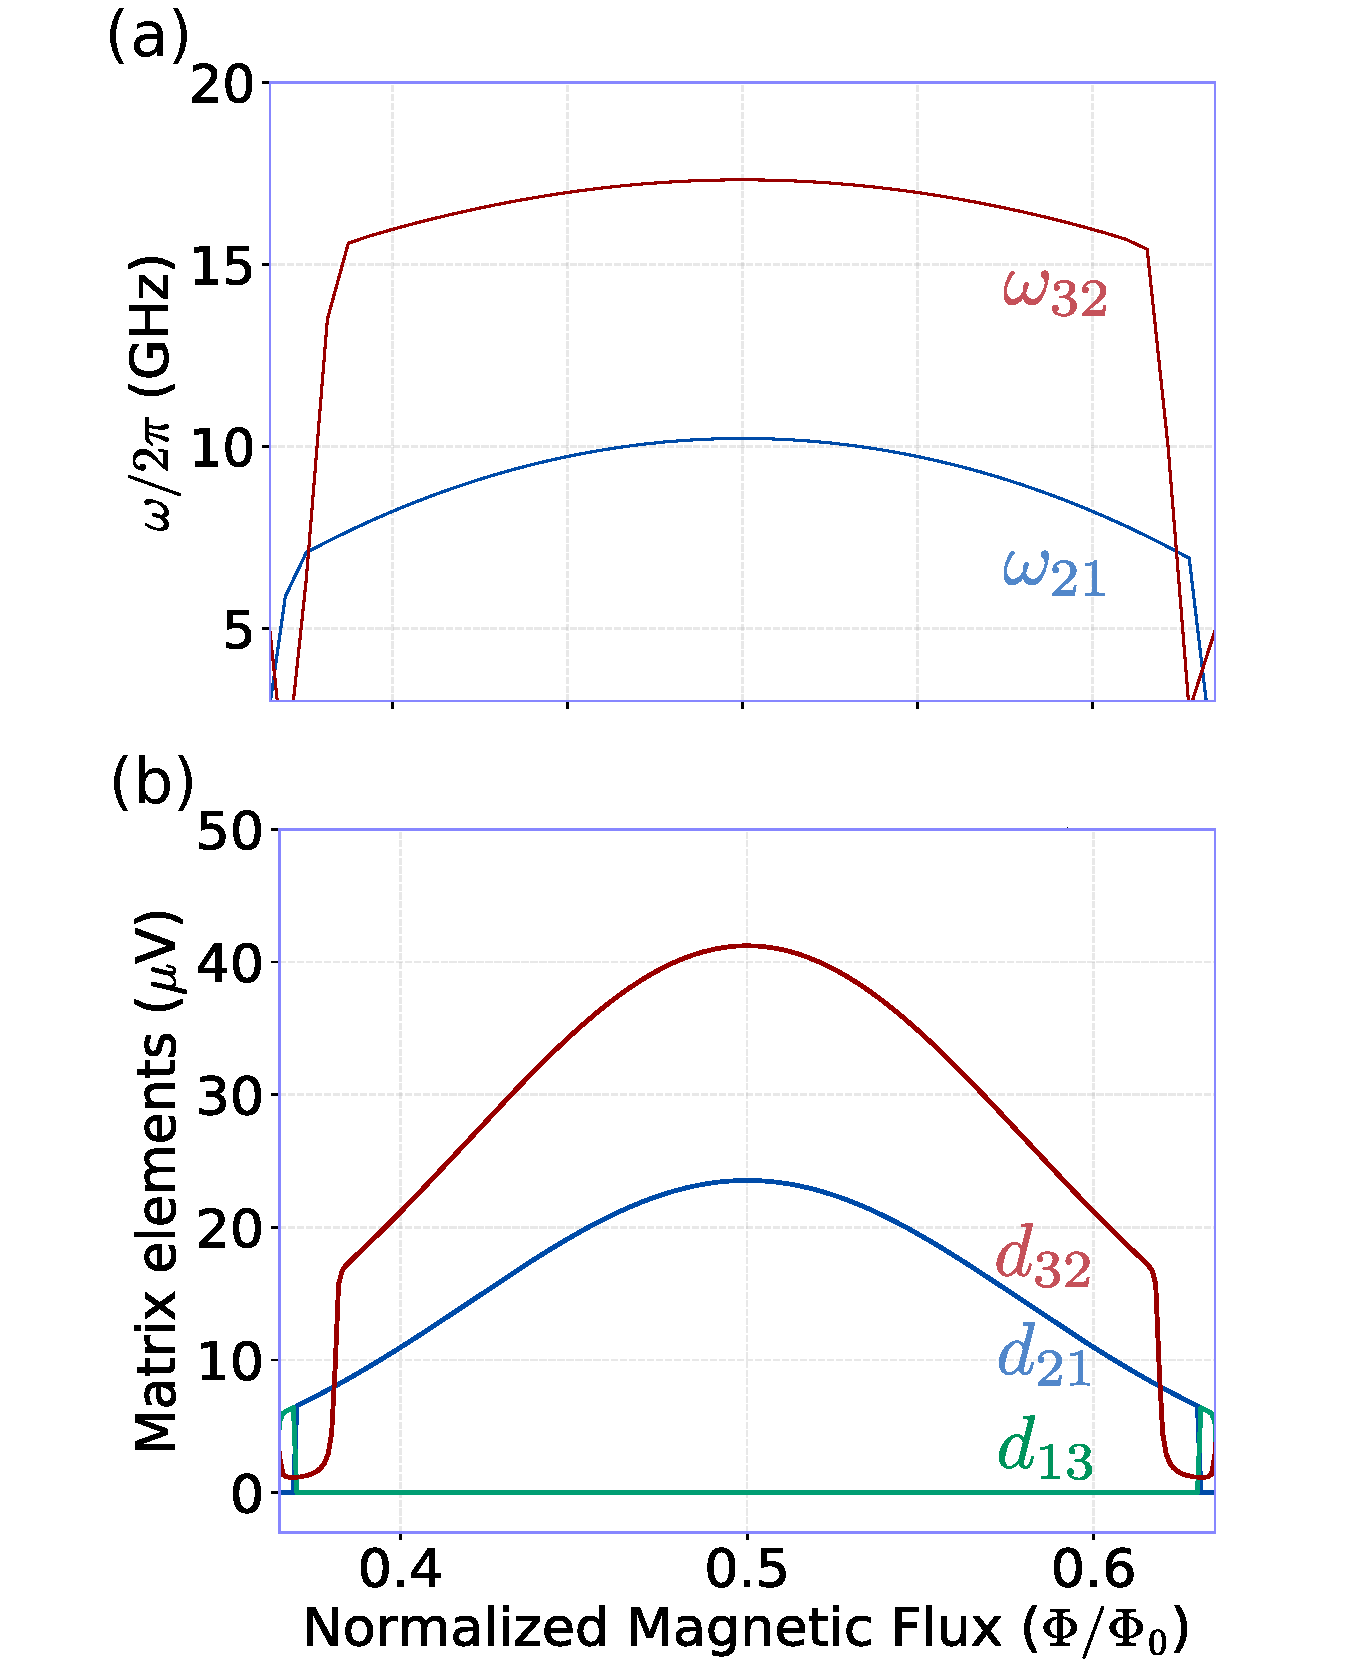
\includegraphics[height=5cm]{fig3}
  \caption{\small \textbf{Experimental spectra,  circles, and simulation, solid  lines, of the
      twin   qubit:}  Shown   are  the   transition  frequencies   $  \omega_{21}   $  (blue)   and
    $ \omega_{32}$ (red). Asymmetry in the flux penetrating the left and right loops results in the
    gradual change of transition frequencies with every $ \Phi_{0} $ period - $\omega_{21}$ creeps up,
    while   $\omega_{32}$  creeps   down,  breaking   the  usual   spectrum  periodicity   of  flux
    qubits.  \label{fig:experiment}}
\end{figure}
 
An important qubit parameter is the curvature at the turning points in the energy spectrum, at
the operation  point of  the qubit.   A low  curvature is  desirable, to  make the  qubit less
sensitive to external flux changes, which would improve decoherence time.  At the twin qubits'
degeneracy  points   $  \Phi  =   (n  +  \frac{1}{2})\Phi_0,   n\in\mathbb{Z}  $,  the   curvature  is
$   -550\pm10\,\text{GHz}/\Phi_0^2  $.    It  is   substantially   smaller  than   $  13\times   10^4$
$ \text{GHz}/\Phi_0^2$ on the 4-JJ flux qubit  \cite{stern2014}, $ 8.4 \times 10^4$ \cite{zhu2010} and
$ 37\times 10^{4}$  $ \text{GHz}/\Phi_0^2$ \cite{gustavsson2012} on the 3-JJ  flux qubits demonstrated
recently.   The decoherence  time of  $ =  \iunit{42}{ns} $,  taken with  Rabi oscillation  in
Fig.~\ref{fig:rabi}   and  described   in  Appendix~\ref{sec:rabi-oscill-meas},   was  however
relatively short.  We attribute  this to poisoning of the sample  with the infrared radiation,
and simplified technology used for the qubit's fabrication.

  \begin{figure}[h]
    \includegraphics[height = 5cm]{fig5}
    \caption{Rabi oscillation taken at the degeneracy point by driving the qubit with resonant
      microwaves  pulses  for  fixed  time  periods,  $  \Delta  t  $.   The  decoherence  time  of
      $   \tau_{\text{dec}}  =   \iunit{42}{ns}  $   is  extracted   from  the   decay  envelope,
      $ e^{-\Delta t/\tau_{\text{dec}}} $, of the the oscillations. \label{fig:rabi}}
  \end{figure}
  % Despite the twin qubit have a much the decoherence time
  % in our qubits was
  % relatively small This improved robustness to flux noise
  % is matched by a
  % decoherence time of , extracted from Rabi oscillations
  % in Fig.~\ref{fig:rabi}
  % \cite{rabi}.

%%% Local Variables:
%%% mode: latex
%%% TeX-master: "../dipole_ilya_paper"
%%% End:
